\chapter{基于深度学习方法的低分辨率环境下微表情识别}\label{chap:owner2}

我们考虑在不受控制的环境中对动作的全自动识别。大多数现有的工作依赖领域知识从输入构建复杂的手工特性。此外,通常假定环境是受控的。卷积神经网络(tional neural network, CNNs)是一种深度模型,
它可以直接作用于原始输入,从而实现特征构造过程的自动化。然而,这些模型目前仅限于处理2D输入。在本文中,我们开发了一种新的三维CNN动作识别模型。该模型通过三维卷积从空间和时间两个维度提取特
征,从而获取多个相邻帧中编码的运动信息。所建立的模型从输入帧中生成多个通道的信息,并结合所有通道的信息得到最终的特征表示。我们将开发的模型应用到现实环境中的人类行为识别中,在不依赖于手工
制作的特性的情况下取得了优异的性能。

Micro-expression is one of important clues for detecting lies. Its most outstanding characteristics include short duration and low intensity of movement. Therefore, video clips of high spatial-temporal resolution are much more desired than still images to provide sufficient details. On the other hand, owing to the difficulties to collect and encode micro-expression data, it is small sample size. In this paper, we use only 560 micro-expression video clips to evaluate the proposed network model: Transferring Long-term Convolutional Neural Network (TLCNN). TLCNN uses Deep CNN to extract features from each frame of micro-expression video clips, then feeds them to Long Short Term Memory (LSTM) which learn the temporal sequence information of micro-expression. Due to the small sample size of micro-expression data, TLCNN uses two steps of transfer learning: (1) transferring from expression data and (2) transferring from single frame of micro-expression video clips, which can be regarded as “big data”. Evaluation on 560 micro-expression video clips collected from three spontaneous databases is performed. The results show that the proposed TLCNN is better than some state-of-the-art algorithms.
微表情是检测谎言的重要线索之一。它最突出的特点是运动时间短,强度低。因此,高时空分辨率的视频片段比静止图像更需要提供足够的细节。另一方面,由于微表达数据的采集和编码困难,样本量较小。在本文中,我们仅使用560个微表情视频片段来评价所提出的网络模型:transfer long tional Neural network (TLCNN)。TLCNN利用深度CNN从微表情视频片段的每一帧中提取特征,然后将其输入到长短时记忆(Long Short-Term Memory, LSTM)中,LSTM学习微表情的时序信息。由于微表情数据的样本容量较小,TLCNN采用了两个迁移学习的步骤:(1)从表情数据进行迁移,(2)从单帧微表情视频片段进行迁移,可视为“大数据”。对采集自三个自发性数据库的560个微表情视频片段进行评价。结果表明,所提出的TLCNN算法优于现有的一些算法。

Recently, owing to the rapid development of computer hardware, especially Graphical Processor Unit (GPU), deep learning is applied on many areas such as face recognition [35] and verification [36], and shows outstanding performances. These deep learning methods use multiple processing layers to discover patterns and structures in very large data sets. Each layer learns a concept from the data that subsequent layers build on; the higher the level, the more abstract the concepts that are learned. Deep learning does not depend on prior data processing and automatically extracts features [37]. These advantages and good performances of deep learning are ascribed to big data. However, the number of micro-expression video clips is usually small. Deep learning on data with small sample size may not achieve good performances. To address this problem, we use transfer learning to pretrain a deep convolutional neural network and we propose the Transferring Long-term Convolutional Neural Network (TLCNN) model for micro-expression recognition. In TLCNN, there are two steps of transfer learning: (1) transferring from expression data and (2) transferring from single frame of micro-expression video clips, which can be regarded as big data . To fully use the temporal information in micro-expression videos, TLCNN also uses Long Short Term Memory (LSTM) to extract temporal features of micro-expression videos from mid-level image representation for each frame images.
近年来,随着计算机硬件特别是图形处理器单元(GPU)的飞速发展,深度学习在人脸识别[35]、验证[36]等领域得到了广泛的应用,表现出了优异的性能。这些深度学习方法使用多个处理层来发现非常大的数据集中的模式和结构。每一层从后续层构建的数据中学习一个概念;层次越高,所学的概念就越抽象。深度学习不依赖于先验数据处理,自动提取特征[37]。这些优势和深度学习的良好表现都归功于大数据。然而,微表情视频剪辑的数量通常很少。在样本容量较小的数据上进行深度学习可能不会取得良好的效果。针对这一问题,我们利用转移学习对深度卷积神经网络进行预处理,提出了用于微表情识别的转移长期卷积神经网络(TLCNN)模型。在TLCNN中,迁移学习有两个步骤:(1)从表达数据进行迁移,(2)从单个微表达视频片段帧进行迁移,这可以看作是大数据。为了充分利用微表情视频中的时间信息,TLCNN还利用长短时记忆(Long Short Term Memory, LSTM)从每帧图像的中层图像表示中提取微表情视频的时间特征。
\section{数据集预处理}

数据增强(Data Augmentation):是指对图片进行随机的旋转、翻转、裁剪、随机设置图片的亮度和对比度以及对数据进行标准化(数据的均值为0,方差为1)。通过这些操作,我们可以获得更多的图片样本,原来的一张图片可以变为多张图片,扩大了样本容量,对于提高模型的准确率和提升模型的泛化能力非常有帮助,在进行数据增强的同时也会需要消耗大量的系统资源。


\subsection{数据集混合}



\subsection{直方图均衡化}

直方图均衡化(Histogram Equalization) 又称直方图平坦化,实质上是对图像进行非线性拉伸,重新分配图像象元值,使一定灰度范围内象元值的数量大致相等。这样,原来直方图中间的峰顶部分对比度得到增强,而两侧的谷底部分对比度降低,输出图像的直方图是一个较平的分段直方图:如果输出数据分段值较小的话,会产生粗略分类的视觉效果。

直方图是表示数字图像中每一灰度出现频率的统计关系。直方图能给出图像灰度范围、每个灰度的频度和灰度的分布、整幅图像的平均明暗和对比度等概貌性描述。灰度直方图是灰度级的函数, 反映的是图像中具有该灰度级像素的个数, 其横坐标是灰度级$r$, 纵坐标是该灰度级出现的频率( 即像素的个数) $p_{r}(r)$, 整个坐标系描述的是图像灰度级的分布情况, 由此可以看出图像的灰度分布特性, 即若大部分像素集中在低灰度区域, 图像呈现暗的特性; 若像素集中在高灰度区域, 图像呈现亮的特性。

图~\ref{fig20}所示就是直方图均衡化, 即将随机分布的图像直方图修改成均匀分布的直方图。基本思想是对原始图像的像素灰度做某种映射变换, 使变换后图像灰度的概率密度呈均匀分布。这就意味着图像灰度的动态范围得到了增加, 提高了图像的对比度。

\begin{figure}[!htb]
\centering
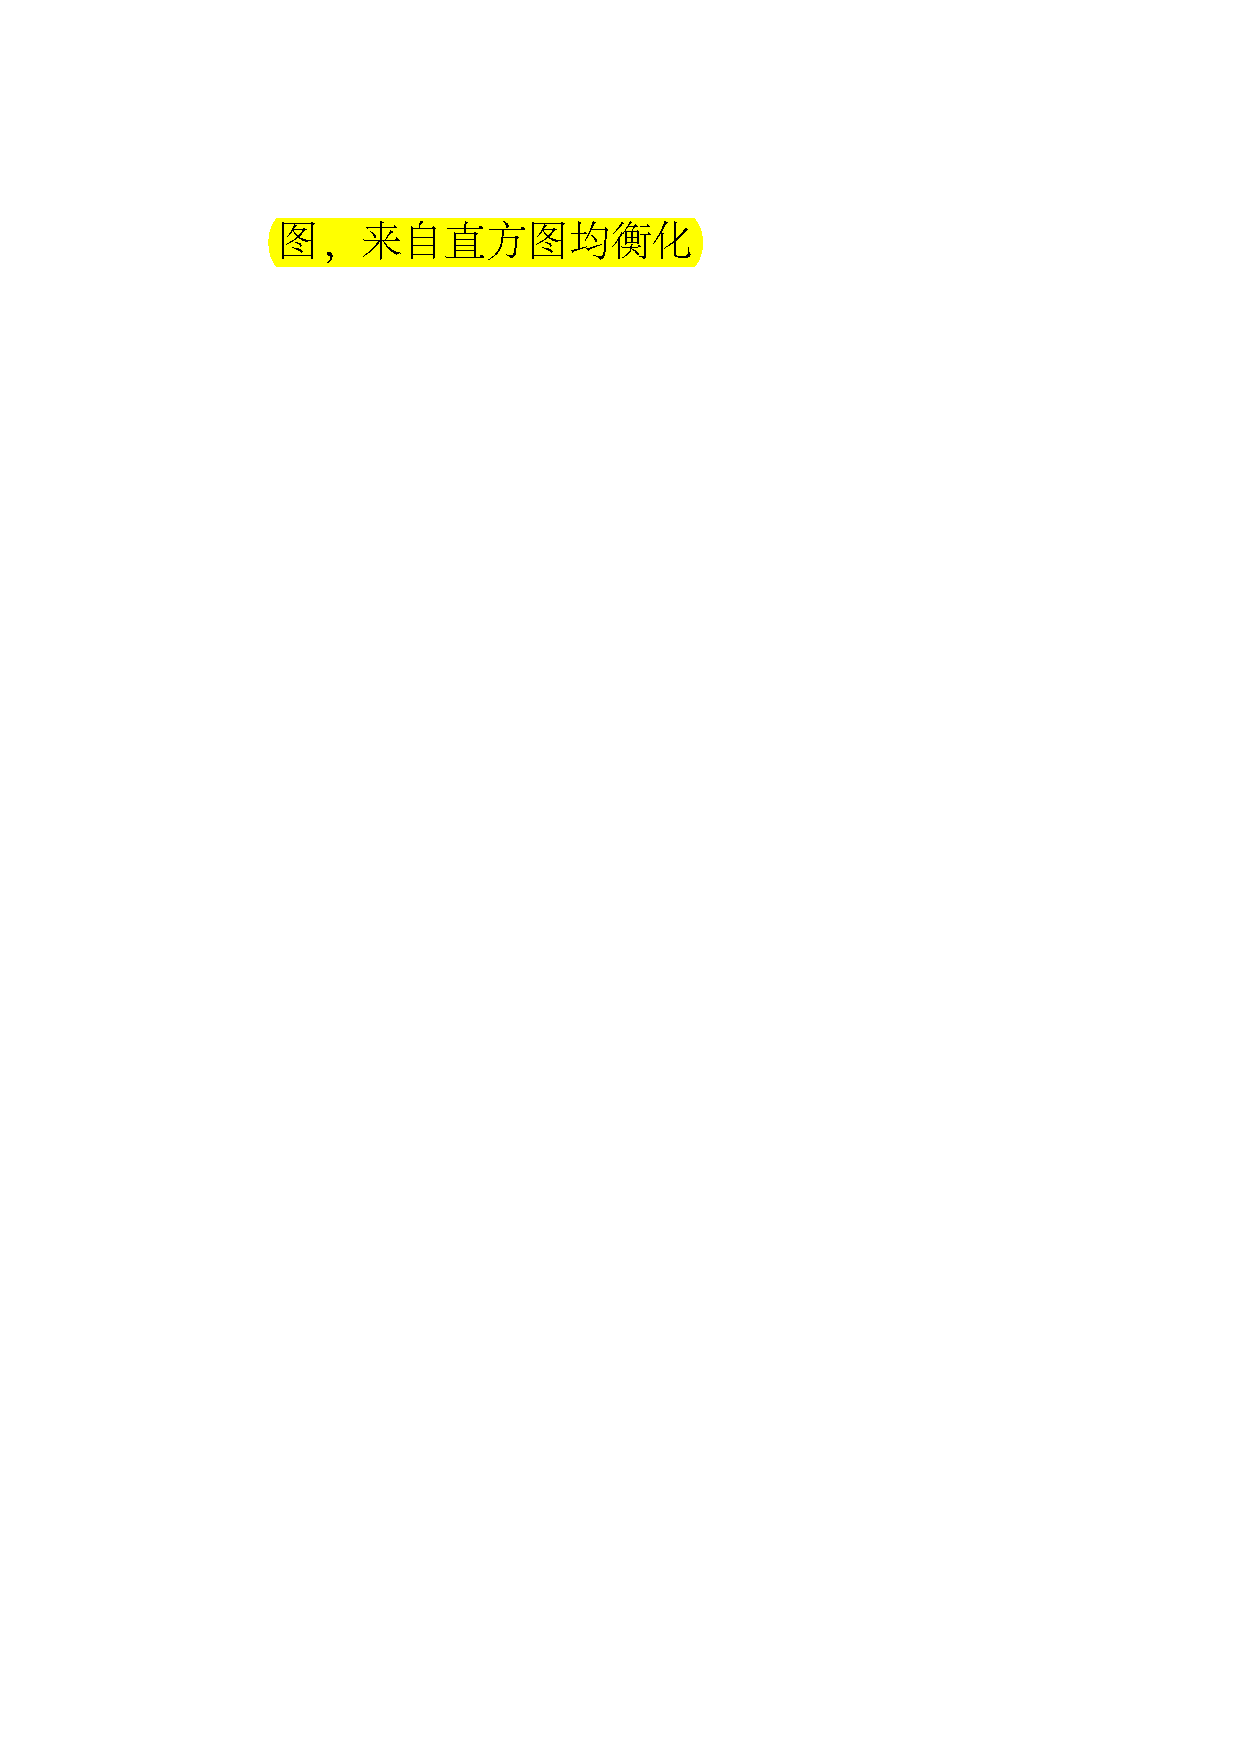
\includegraphics[width=0.75\textwidth]{4LR1}
\caption{直方图均衡化}
\label{fig20}
\end{figure}

通过这种技术可以清晰地在直方图上看到图像亮度的分布情况, 并可按照需要对图像亮度调整。另外,这种方法是可逆的, 如果已知均衡化函数, 就可以恢复原始直方图。

设变量$r$代表图像中像素灰度级。对灰度级进行归一化处理, 则$0\leqslant r\leqslant 1$ , 其中$r=0$表示黑,$r=1$表示白。对于一幅给定的图像来说, 每个像素值在[0,1]的灰度级是随机的。用概率密度函数$p_{r}(r)$ 来表示图像灰度级的分布。

为了有利于数字图像处理, 引入离散形式。在离散形式下, 用$r^{k}$ 代表离散灰度级, 用$p_{r}(r^{k})$ 代表$p_{r}(r)$ , 并且下式成立:$p_{r}(r^{k})=nk/n$,其中,$0\leqslant r^{k}\leqslant 1$,$k=0,1,2,\cdots ,n-1$ 。式中$n^{k}$为图像中出现$r^{k}$这种灰度的像素数, $n$是图像中的像素总数, 而$nk/n$就是概率论中的频数。图像进行直方图均衡化的函数表达式为:
\begin{equation}
 \label{eq6}
 \begin{split}
   S_{i}=T(r_{i})=\sum_{i=0}^{k-1}\frac{n_{i}}{n}
 \end{split}
\end{equation}
式中, $k$为灰度级数。相应的反变换为:
\begin{equation}
 \label{eq6}
 \begin{split}
   r^{i}=T^{-1}(S_{i})
 \end{split}
\end{equation}

\subsection{亮度调整}



\section{特征提取及识别}

\subsection{P3D 块}

Inspired by the recent successes of Residual Networks (ResNet) [7] in numerous challenging image recognition tasks, we develop a new family of building modules named Pseudo-3D (P3D) blocks to replace 2D Residual Units in ResNet, pursuing spatio-temporal encoding in ResNet-like architectures for videos. Next, we will recall the basic design of Residual Units in ResNet, followed by presenting how to devise our P3D blocks. The bottleneck building architecture on each P3D block is finally elaborated.
受最近残差网络(ResNet)[7]在众多具有挑战性的图像识别任务中取得的成功启发,我们开发了一个名为伪3d (P3D)块的构建模块家族,以取代ResNet中的2D残差单元,在视频的ResNet-like架构中实现时空编码。接下来,我们将回顾ResNet中剩余单元的基本设计,然后介绍如何设计P3D块。最后阐述了每个P3D块上的瓶颈构建体系结构。

Residual Units
残差单位
ResNet consists of many staked Residual Units and each Residual Unit could be generally given by
ResNet由许多桩状残余单元组成,每个残余单元通常由eq (1)
\begin{equation}
\label{eq6}
   \textbf{x}_{t+1}=\textbf{h}(\textbf{x}_{t})+\textbf{F}(\textbf{x}_{t})
\end{equation}
where xt and xt+1 denote the input and output of the t-th Residual Unit, h (xt) = xt is an identity mapping and F is a non-linear residual function. Hence, Eq.(1) can be rewritten as

其中$\textbf{x}_{t}$和$\textbf{x}_{t+1}$表示第$t$个残差单元的输入和输出,$\textbf{h}(\textbf{x}_{t})=\textbf{x}_{t}$为恒等映射,$\textbf{F}$为非线性残差函数。因此,式(1)可以改写为eq(2)
where F · xt represents the result of performing residual function F over xt. The main idea of ResNet is to learn the additive residual function F with reference to the unit inputs xt which is realized through a shortcut connection, instead of directly learning unreferenced non-linear functions.
\begin{equation}
\label{eq6}
   (\textbf{I}+\textbf{F})\cdot \textbf{x}_{t}=\textbf{x}_{t}+\textbf{F}\cdot \textbf{x}_{t}:=\textbf{x}_{t}+\textbf{F}(\textbf{x}_{t})=\textbf{x}_{t+1}
\end{equation}
其中$\textbf{F})\cdot \textbf{x}_{t}$表示在$\textbf{x}_{t}$上执行残差函数$\textbf{F}$的结果。ResNet的主要思想是通过一个快捷的连接,而不是直接学习未引用的非线性函数,来学习参考单元输入$\textbf{x}_{t}$的可加性残差函数$\textbf{F}$。

P3D Blocks design
P3D块设计

To develop each 2D Residual Unit in ResNet into 3D architectures for encoding spatiotemporal video information, we modify the basic Residual Unit in ResNet following the principle of Pseudo 3D as introduced in Section 3.1 and devise several Pseudo-3D Blocks. The modification is not straightforward for involvement of two design issues. The first issue is about whether the modules of 2D filters on spatial dimension (S) and 1D filters on temporal domain (T) should directly or indirectly influence each other. Direct influence within the two types of filters means that the output of spatial 2D filters is connected as the input to the temporal 1D filters (i.e., in a cascaded manner). Indirect influence between the two filters decouples the connection such that each kind of filters is on a different path of the network (i.e., in a parallel fashion). The second issue is whether the two kinds of filters should both directly influence the final output. As such, direct influence in this context denotes that the output of each type of filters should be directly connected to the final output.
为了将ResNet中的每个2D残差单元发展成用于编码时空视频信息的3D架构,我们按照3.1节中介绍的伪3D原理对ResNet中的基本残差单元进行了修改,并设计了几个伪3D块。由于涉及两个设计问题,所以修改并不简单。第一个问题是空间维度上的二维滤波器模块和时间域上的一维滤波器模块是否应该直接或间接地相互影响。两种滤波器之间的直接影响是将空间二维滤波器的输出连接为时间一维滤波器的输入(即,以级联的方式)。两个过滤器之间的间接影响使连接解耦,使每一种过滤器在网络的不同路径上(即)。第二个问题是这两种过滤器是否都应该直接影响最终的输出。因此,在此上下文中,直接影响表示每种过滤器的输出都应该直接连接到最终输出。

Based on the two design issues, we derive three different P3D blocks as depicted in Figure 2, respectively, named as P3D-A to P3D-C. Detailed comparisons about their architectures are provided as following:
基于这两个设计问题,我们推导出如图2所示的三个不同的P3D块,分别命名为P3D- a到P3D- c。关于它们的架构的详细比较如下:

(1) P3D-A: The first design considers stacked architecture by making temporal 1D filters (T) follow spatial 2D filters (S) in a cascaded manner. Hence, the two kinds of filters can directly influence each other in the same path and only the temporal 1D filters are directly connected to the final output, which could be generally given by
eq (3)
(1) P3D-A:第一种设计考虑了层叠结构,使时间一维滤波器(T)以级联方式跟随空间二维滤波器(S)。因此,两种滤波器在同一路径上可以直接相互影响,只有时间1D滤波器直接连接到最终输出,一般可以给出eq(3)

(2) P3D-B: The second design is similar to the first one except that indirect influence between two filters are adopted and both filters are at different pathways in a parallel fashion. Although there is no direct influence between S and T, both of them are directly accumulated into the final  output, which could be expressed as
eq (4)
(2) P3D-B:第二种设计与第一种设计相似,只是采用了两个滤波器之间的间接影响,两个滤波器以并行的方式在不同的路径上。虽然S和T之间没有直接的影响,但是它们都直接累加到最终输出中,可以表示为eq (4)

(3) P3D-C: The last design is a compromise between P3D-A and P3D-B, by simultaneously building the direct influences among S, T and the final output. Specifically, to enable the direct connection between S and final output based on the cascaded P3D-A architecture, we establish a shortcut connection from S to the final output, making the output xt+1 as
eq (5)
(3) P3D-C:最后的设计是在P3D-A和P3D-B之间进行折衷,同时建立S、T和最终输出之间的直接影响。具体来说,为了基于级联P3D-A架构实现S与最终输出的直接连接,我们建立了S到最终输出的快捷连接,使输出xt+1为eq(5)

Bottleneck architectures
瓶颈的架构

When specifying the architecture of 2D Residual Unit, the basic 2D block is modified with a bottleneck design for reducing the computation complexity. In particular, as shown in Figure 3(a), instead of a single spatial 2D filters (3 3 convolutions), the Residual Unit adopts a stack of 3 layers including 1 1, 3 3, and 1 1 convolutions, where the first and last 1 1 convolutional layers are applied for reducing and restoring dimensions of input sample, respectively. Such bottleneck design makes the middle 3 3 convolutions as a bottleneck with smaller input and output dimensions. Thus, we follow this elegant recipe and utilize the bottleneck design to implement our proposed P3D blocks. Similar in spirit, for each P3D block which purely consists of one spatial 2D filters (1 3 3 convolutions) and one temporal 1D filters (3 1 1 convolutions), we additionally place two 1 1 1 convolutions at both ends of the path, which are responsible for reducing and then increasing the dimensions. Accordingly, the dimensions of the input and output of both the spatial 2D and temporal 1D filters are reduced with this bottleneck design. The detailed bottleneck building architectures on all the three P3D blocks are illustrated in Figure 3(b) to 3(d).
在确定二维残差单元的体系结构时,对二维基本块进行瓶颈设计,以降低计算复杂度。特别是,如图3所示(一个),而不是一个单一的空间2 d过滤器(3 3旋转),剩余单位采用一堆3层包括1 1 3 3 1 1曲线玲珑,第一个和最后一个1 1卷积层在哪里申请减少和恢复方面的输入样本,分别。这样的瓶颈设计使得中间的3 3个卷积成为输入和输出维数较小的瓶颈。因此,我们遵循这个优雅的配方,并利用瓶颈设计来实现我们提出的P3D块。相似的精神,为每个P3D块纯粹由一个空间二维滤波器卷积(1 3 3)和一个时间1 d过滤器(3 1 1旋转),我们另外两个1 1 1两端的卷积路径,负责降低,然后增加尺寸。因此,该瓶颈设计减少了空间二维和时间一维滤波器的输入和输出的维数。图3(b) - 3(d)展示了这三个P3D块上详细的瓶颈构建体系结构。

\subsection{P3D ResNet}

In order to verify the merit of the three P3D blocks, we first develop three P3D ResNet variants, i.e., P3D-A ResNet, P3D-B ResNet and P3D-C ResNet by replacing all the Residual Units in a 50-layer ResNet (ResNet-50) [7] with one certain kind of P3D block, respectively. The comparisons of performance and time efficiency between the basic ResNet-50 and the three P3D ResNet variants are presented. Then, a complete version of P3D ResNet is proposed by mixing all the three P3D blocks from the viewpoint of structural diversity.
为了验证这三个P3D模块的优点,我们首先开发了三个P3D ResNet变体,即, P3D- a ResNet、P3D- b ResNet和P3D- c ResNet分别用一种P3D块替换50层ResNet (ResNet-50)[7]中的所有残余单元。比较了基本ResNet-50和三种P3D ResNet变体的性能和时间效率。然后,从结构多样性的角度,将三个P3D块混合在一起,提出了一个完整的P3D ResNet版本。

Mixing different P3D Blocks. Further inspired from the recent success of pursuing structural diversity in the design of very deep networks [38], we devise a complete version of P3D ResNet by mixing different P3D blocks in the architecture to enhance structural diversity, as depicted in Figure 4. Particularly, we replace Residual Units with a chain of our P3D blocks in the order P3D-A->P3D-B->P3D-C. Table 1 also details the performance and speed of the complete P3D ResNet. By additionally pursuing structural diversity, P3D ResNet makes the absolute improvement over P3D-A ResNet, P3D-B ResNet and P3D-C ResNet by 0.5\%, 1.4\% and 1.2\% in accuracy respectively, indicating that enhancing structural diversity with going deep could improve the power of neural networks.
混合不同的P3D块。从最近在深度网络[38]的设计中追求结构多样性的成功中得到进一步的启发,我们设计了一个完整的P3D ResNet版本,通过在架构中混合不同的P3D块来增强结构多样性,如图4所示。特别地,我们用P3D- a ->P3D- b ->P3D- c顺序的P3D区块链替换剩余的单元。表1还详细说明了完整P3D ResNet的性能和速度。通过进一步追求结构多样性,P3D ResNet相对于P3D- a ResNet、P3D- b ResNet和P3D- c ResNet的准确率分别提高了0.5\%、1.4\%和1.2\%,说明随着深度的增加,结构多样性的增强可以提高神经网络的能力。

在视频分类或理解领域,容易从图像领域的2D卷积联想到用3D卷积来做,虽然用3D卷积进行特征提取可以同时考虑到spatial和temporal维度的特征,但是计算成本和模型存储都太大,因此这篇文章针对视频领
域中采用的3D卷积进行改造,提出Pseudo-3D Residual Net (P3D ResNet),思想有点像当年的Inception v3中用1*3和3*1的卷积叠加代替原来的3*3卷积,这篇文章是用1*3*3卷积和3*1*1卷积代替3*3*3卷
积(前者用来获取spatial维度的特征,实际上和2D的卷积没什么差别;后者用来获取temporal维度的特征,因为倒数第三维是帧的数量),毕竟这样做可以大大减少计算量,而如果采用3D卷积来做的话,速度
和存储正是瓶颈,这也使得像C3D算法的网络深度只有11层,参看Figure1。该文章的网络结构可以直接在3D的ResNet网络上修改得到。顺便提一下,除了采用3D卷积来提取temporal特征外,还可以采用LSTM来
提取,这也是当前视频研究的一个方向。

Figure1是几个模型在层数、模型大小和在Sports-1M数据集上的视频分类效果对比,其中的P3D ResNet是在ResNet 152基础上修改得到的,深度之所以不是152,是因为改造后的每个residual结构不是原
来ResNet系列的3个卷积层,而是3或4个卷积层,详细可以看Figure3,所以最后网络深度是199层。官方github代码中的网络就是199层的。ResNet 152是直接在Sports-1M数据集上fine tune得到的。可
以看出199层的P3D ResNet虽然在模型大小上比ResNet-152(此处ResNet-152是在sports-1M数据集上fine tune得到的)大一些,但是准确率提升比较明显,与C3D(此处C3D是直接在sports-1M数据集
上从头开始训练得到的)的对比在效果和模型大小上都有较大改进,除此之外,速度的提升也是亮点,后面有详细的速度对比。

\begin{figure}[]
\centering
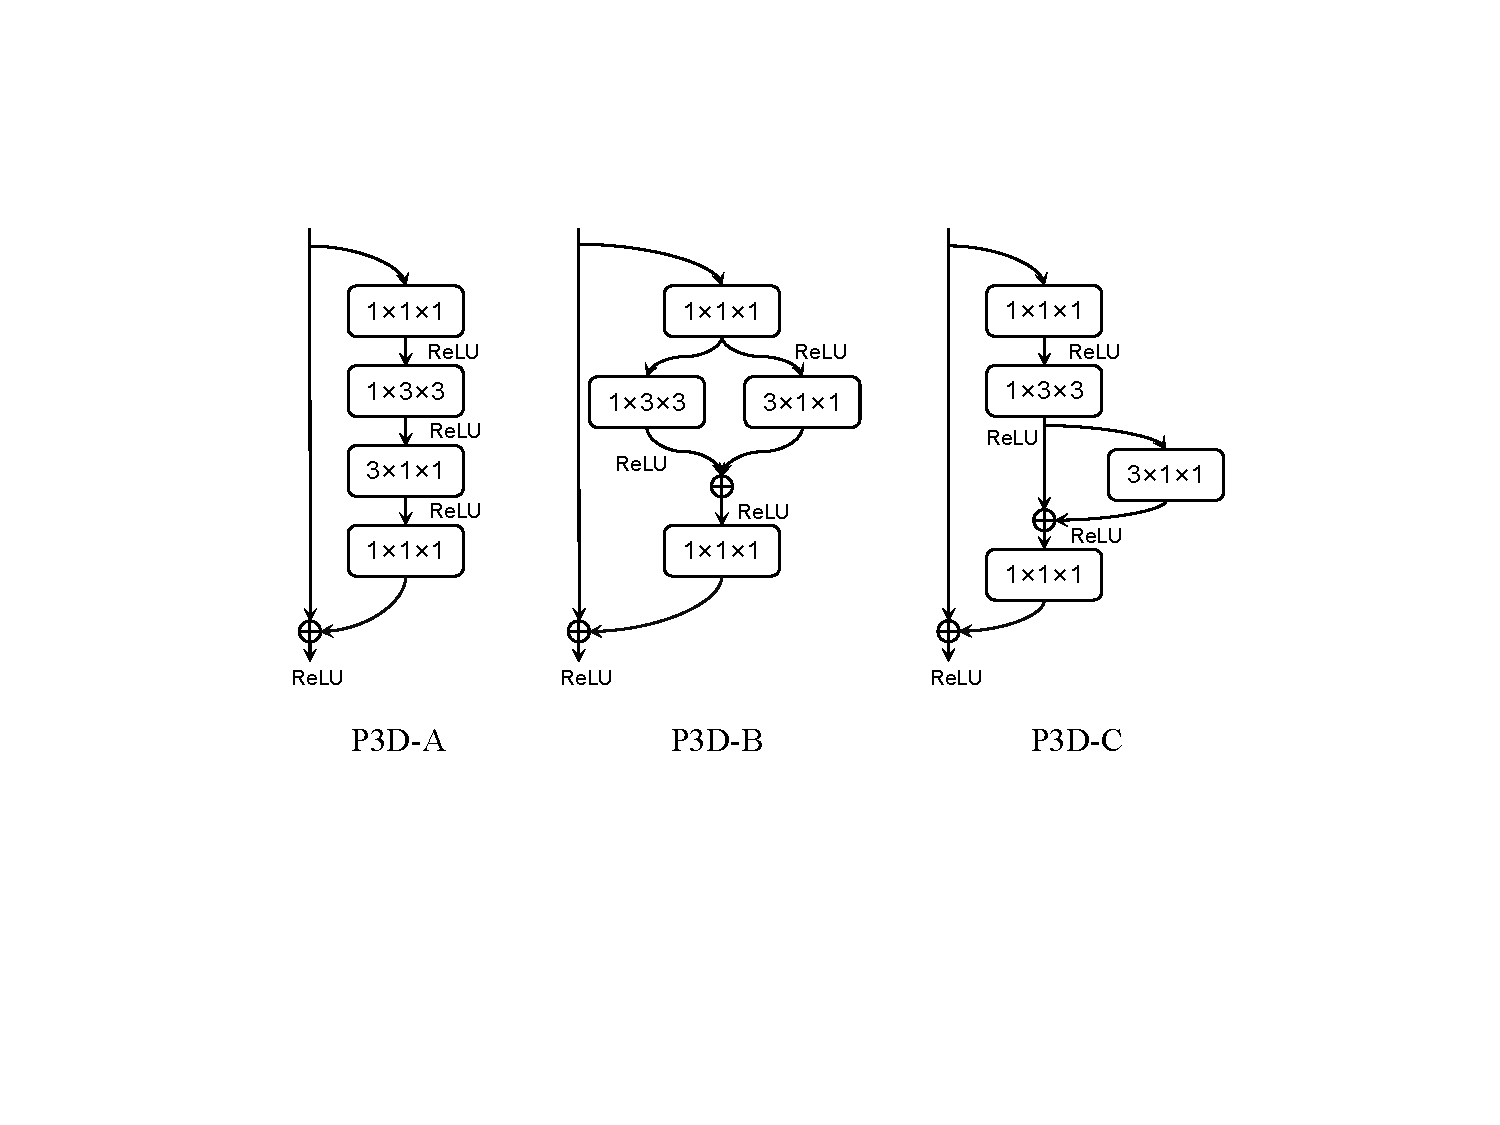
\includegraphics[width=0.75\textwidth]{P3D0}
\caption{伪3D残差网络三种设计模型}
\label{fig18}
\end{figure}

\subsection{2}



\section{实验设置及分析}

\subsection{1}

\subsection{2}

\subsection{3}

\section{总结}
